\documentclass[a4paper]{report}

\usepackage[english]{babel}
\usepackage[utf8]{inputenc}
\usepackage{amsmath}
\usepackage{graphicx}
\usepackage[colorinlistoftodos]{todonotes}
\usepackage[colorlinks]{hyperref}

\title{A Cryptographically Protected Phone System}

\author{Andres Erbsen and Adam Yedidia}

\date{\today}

\begin{document}
\maketitle

\section*{Introduction}

In today's excessively monitored and public world, there is no more privacy. An
email can be read by Google, and a chat conversation can be read by Facebook. A
conversation over a cell phone can be intercepted at a cell phone tower, and a
phone conversation over a landline can be wiretapped. In the era of technology,
there is no longer a way to communicate privately except face-to-face.

No way, that is, except for cryptographically protected communications. The last
century, in addition to bringing about the technologies mentioned above for
communicating remotely (along with the technologies used to eavesdrop on them)
also brought about the invention of clever cryptographic schemes for hiding
information securely. These schemes go by many names; in our implementation, we
made use of a particular implementation: the one called Diffie-Hellman-Merkle key
exchange. Diffie-Hellman-Merkle key exchange begins with what we call a ``handshake'' between the two parties; an initialization phase that involves the two participants agreeing to a shared key, which will % this will is intentional
determine the encryption protocol. The truly incredible thing about the Diffie-Hellman-Merkle handshake (along
with a handful of other schemes which we did not use) is that it enables two
interlocutors \emph{with no prior agreements or contact} to communicate securely
in the presence of an eavesdropper \emph{who can hear everything they ever say
to each other, including the entire handshake}[1][2]. Conditioned on the hardness of various problems which are widely
believed to in fact be very difficult to solve by the wider academic community,
it is in fact provably intractable for the eavesdropper to hear the
communications[3].

In what follows, we will % this will is intentional
give a detailed description a hardware implementation of a telephone
system that is cryptographically protected in a theoretically defensible
way; that is, for an attacker to be able to eavesdrop on a call using our
telephone system would require either a long-standing conjecture to be false, or
would require more vastly more computational power than is available to the
world today. We begin this report with a high-level description of the ideas and concepts behind what we did; in the second half of the report, we give more low-level, detailed descriptions of how we actually implemented all the high-level ideas, and the challenges we encountered in that process.

At various points in this paper, we will % this will is intentional
find it convenient to describe two hypothetical users of our system, and a hypothetical attacker; in general, we will % this will is intentional
use the names Alice and Bob to designate the legitimate users, and Eve to designate the eavesdropper.

\chapter{High-Level Description}

\section{Transmitting Audio}

In order to transmit the audio across the channel, we organize the audio
signal into packets, to be sent one at a time across the channel. It is more
efficient to perform the cryptographic calculations when the input is in
available in larger chunks than a single audio sample. Packets come in two types: audio packets and handshake packets, depending on whether or not the two participants in the conversation have already successfully contained the Diffie-Hellman-Merkle handshake. Each packet
contains a header, which serves the purpose of informing the recipient that the packet has begun. Audio packets also contain a sequence number and the audio data; handshake packets also contain a public key and information about whether or not the other person's public key has already been received. 

In order to assemble a packet, we have a buffer module which 
accumulates the bits before sending them all at once in packet form. The buffer
makes use of the BRAMs in order to be as efficient as possible, and because
it is storing a potentially large amount of memory (so simply using
flip-flops would be a waste of valuable programmable logic).

Finally, the packets themselves are transmitted over a simple wire that
connects two FPGA labkits, after having been encrypted by the encryption module.
The wire is long and has a certain amount of noise, so we oversample (look at the value on the wire multiple times) to make reading errors much less likely than they otherwise would be.

\section{Cryptographic protection}

As it is easy for an individual to come up with a cryptosystem that they
themselves cannot break, but harder to create one that will % this will is intentional
withstand attacks
from others, we based our design on existing well-audited building
blocks. As we are not aware of any freely available Verilog implementations of
these algorithms, we implemented them and verified their correctness by
comparing the behavior of our hardware implementations to the existing reference
(software) implementations.

The overall plan is as follows: in the very beginning of each call, the two
communicating labkits perform a Diffie-Hellman-Merkle handshake to generate a
shared secret. That secret is used to seed a pseudo-random keystream
generator and the digital audio signal will be xor-ed with the keystream.
This prevents the attacker (who does not know the shared secret or the
keystream) from recovering the audio signal. 

\begin{description}
  \item[Call Initialization:] Participant A chooses random $a$ and reveals $g^a$,
	  B chooses $b$, reveals $g^b$; both compute $s=g^{ab}$. $g$ is a public constant.
  \item[Encryption:] $\text{encrypted}_i = \text{data}_i \mathbin{\oplus} \text{keystream}(s,i)$
  \item[Decryption:] $\text{data}_i = \text{encrypted}_i \mathbin{\oplus} \text{keystream}(s,i)$
  \item[Packetization:] $\text{packet}_i = \left(type, i, \text{length}(\text{encrypted}_i), \text{encrypted}_i\right)$
  \item[Authentication:] $\text{authenticator}_i = \text{hash}(s, \text{packet}_i)$
  \item[Auth. checking:] Accept received packet iff $\text{hash}(s, \text{packet}_i) = \text{authenticator}_i$.
\end{description}

The described mechanisms are sufficient against an attacker that can not only see
what is sent over the wire but tamper with it; for example, one might cut the
wire and connect it to their phone instead and all this would continue without
interruption. Furthermore, they might make another call to the intended
recipient and connect these calls while maintaining the ability to eavesdrop. Currently, our labkits display the shared key $g^{ab}$ on them; it would be more secure to change this to displaying a hash of the interlocutor's public key, to
make sure that the two users of ours system are indeed on the same call (and
thus not eavesdropped on). Fortunately, this can easily be done with a one-line change to the inputs to the hex display; we felt that displaying the shared key would be more interesting for the demonstration, because it shows that the two participants have successfully agreed upon a shared protocol. 

As classical Diffie-Hellman-Merkle requires hundreds of modular arithmetic operations
on multiple-thousand-bit numbers to be secure, we use a modern
variation where every modular multiplication is replaced with the addition of
two points on a carefully chosen elliptic curve. The other relevant properties
of elliptic curve addition are the same as for modular multiplication, we will % this will is intentional
even continue to use the classical notation. Even though one elliptic curve
addition uses more than one modular multiplication, smaller numbers can be used
without compromising security. Our choice of primitives goes as follows:

\begin{description}
  \item[Random numbers:] Hash of 100ms of microphone input.
  \item[Diffie-Hellman-Merkle function:] Curve25519[8] (uses arithmetic modulo $2^{255}-19$)
  \item[Keystream:] ChaCha20[5] (uses 32-bit addition, xor, and rotation by constant).
  \item[Hash:] BLAKE (uses 32-bit addition, xor, and rotation by constant).
\end{description}

\section{Resulting User Experience}

Two labkits are connected with a couple of wires. When a connection is
established, both hex displays show the same value. Anything spoken into one
labkit's microphone is heard from the headphones of the other and vice versa.

\section{Possible Attacks}

It is the nature of practical cryptography that it is very difficult to prove the security of your system. In order to prove that nobody can break your encryption in any way, it would be necessary to prove something about the entire space of possible attacks, which is too great to comprehend, or it would be necessary to enumerate every possible attack to the system and show that each fails, which is impossible. Unfortunately, the best we can do at this point is enumerate all widely-known attacks against cryptographic systems, and explain why each one cannot succeed against our system. It is possible (even likely) that there exists some attack not described here that would break our system; unfortunately, the best measure of security that we can offer against such an attack is that because people as a whole haven't thought of it yet, it's likely that a potential attacker wouldn't either.

\subsection{Brute-Force Attacks} 

This class of possible attacks has as its goal to learn through algorithmic means either of the interlocutors' secret keys, which is enough to let the attacker compute the shared secret and the decryption of the message. Assuming that division in the space of elliptic curve functions is computationally difficult (which is widely believed in the academic community to be true) this class of possible attacks won't succeed against our system because of the fact that the only algorithms able to find an interlocutor's secret key as a function of their public key take exponential time; moreover, our key length is long enough that no implementation of any algorithm has come close to being able to do this.

\subsection{Man-in-the-Middle Attacks}

This type of attack is based off the idea of spoofing the two interlocutors into thinking that they are talking to each other, when in fact, they are both talking to the attacker and the attacker is relaying messages between them. No amount of security on the channel itself can protect against an attack of this kind, since the attacker's ability to hear the communications comes from the fact that two participants in a phone conversation can hear the communications--something that is necessary for the basic functioning of a telephone system. However, we can give t the interlocutors the ability to know when there is a man-in-the-middle attacker, by giving everyone access to the public key of a given other person, and also giving them access to the public key of the person they're talking to. If the Alice believes herself to be speaking to Bob, but is actually speaking to Eve, who is executing a man-in-the-middle attack, then she will % this will is intentional
see both Bob and Eve's public keys displayed on her phone's screen, and this will % this will is intentional
tell her that she is not speaking to the person she think she is. This is the basic idea; in reality, we would display not the public key itself (which is much too long to display) but a hash thereof, and if Bob and Eve's public keys were different, then the hashes would be virtually certain to also be different, assuming we used a cryptographic hash function (a hash function which is computationally difficult to invert).

\subsection{Data Manipulation Attacks}

These attacks consist of manipulating the data cleverly; for example, it might be imagined that in an insecure cryptographic system, an attacker might be able to compute the \verb|XOR| of the data on the wire from Alice to Bob and the wire from Bob to Alice, for example, and thereby gain information. Another common potential attack is to compute the \verb|XOR| of the data on the wire with what the data was on the wire in the past. 

These attacks won't work against our system, because of the security guarantees of the Chacha20 hash function; given the output of the hash function on one value, it is computationally difficult to predict the output of the hash function on some different value, and in general the Chacha20 hash function produces values that appear to have no structure. This means that performing arithmetic operations on different snapshots of the encrypted data won't give an attacker any useful information about what's being said.

However, there is another kind of attack which our system is vulnerable to; if Alice is speaking to Bob and Eve has compromised the wire, Eve could move packets around on the wire, or could even remove the packets altogether and replace them with her own, encrypting them to Bob's public key. This does not allow Eve to find out anything about what Alice and Bob are saying, so privacy is preserved, but it does allow Eve to make Alice appear to things that she didn't actually say.

To protect against this attack, a good next step would be to cryptographically sign each packet. This would be a good future avenue for improvement.

\chapter{Detailed Implementation}

In this section, we give a detailed description of our design and how it works. In the pages that follow, we provide two block diagrams that provide a visual summary of our design. In the text, we describe in detail the working of each of the modules shown in the block diagram.

Our implementation is split into two ``phases'': Phase 1, in which the handshake takes place, and Phase 2, in which sound is exchanged between the two users and the phone conversation takes place.

\begin{figure}
\label{fig3}
\makebox[\textwidth][c]{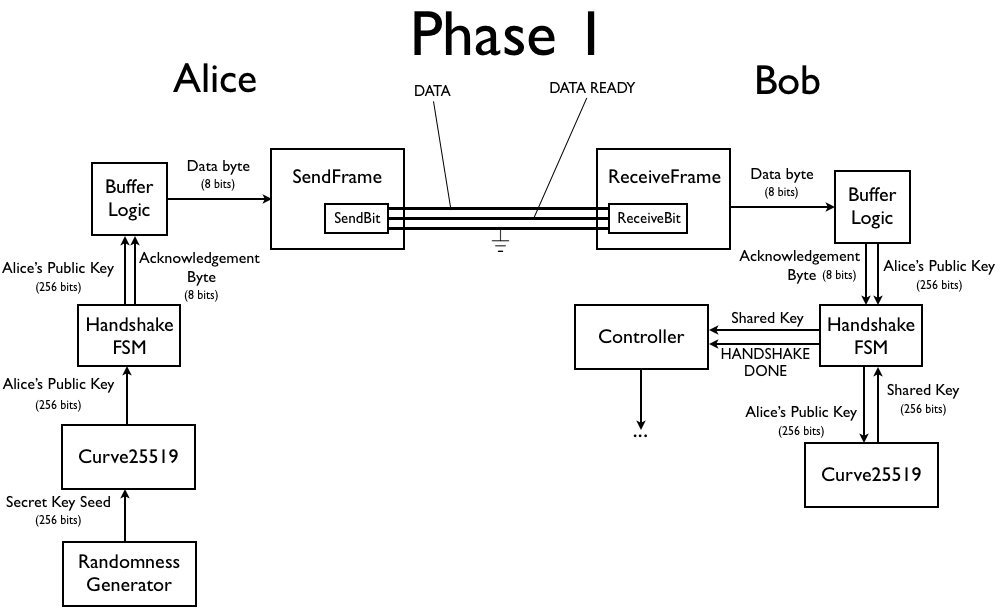
\includegraphics[width=1.7\textwidth]{figs/phase1.png}}%
\centering \caption{A block diagram of the execution of Phase 1. Thick lines indicate external wires (which the attacker has access to), whereas arrows indicate internal wires (which the attacker does not have access to). For clarity, we show only the information flowing from Alice to Bob; in reality, this entire design is duplicated in the other direction.}
\end{figure}

\begin{figure}
\label{fig3b}
\makebox[\textwidth][c]{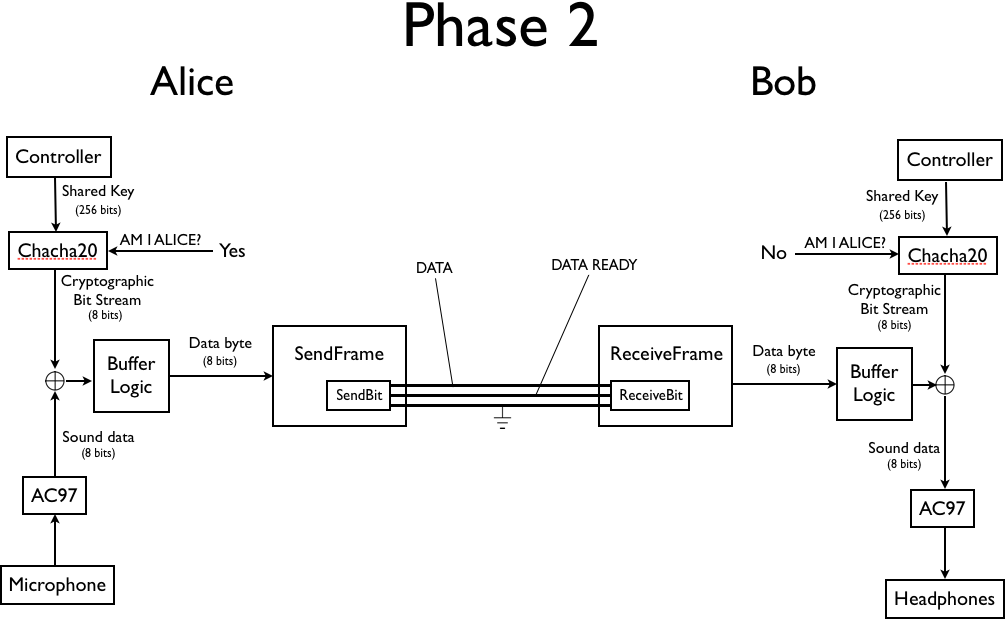
\includegraphics[width=1.7\textwidth]{figs/phase2.png}}%
\centering \caption{A block diagram of the execution of Phase 2. Thick lines indicate external wires (which the attacker has access to), whereas arrows indicate internal wires (which the attacker does not have access to). For clarity, we show only the information flowing from Alice to Bob; in reality, this entire design is duplicated in the other direction.}
\end{figure}

\section{Controller}

\emph{Author of section: Adam Yedidia. The module was jointly designed.} \\

This part of the code did not have its own module, nor did it consist of very much distinct code; however, it is present in the block diagram as a design abstraction, which controls the flow of the system from Phase 1 (handshake) into Phase 2 (audio). Upon turning on the labkit, it tells the Handshake FSM module to begin the handshake; upon successful completion of the handshake, it takes the shared key output by the Handshake FSM module, feeds it into the Chacha20 module, and begins Phase 2. It can be thought of as a very high-level state machine with two states over the entire design.

\section{Handshake FSM}

\emph{Author of section: Adam Yedidia} \\

This module is a finite-state machine in charge of making sure of the proper execution of the Diffie-Hellman-Merkle handshake that communicates the shared key to both participants. It consists of the following seven states, each one leading directly into the next: \\ \\
1. Waiting for start pulse: the state machine is idle and waiting to be told to begin. \\
2. Computing the public key: the state machine takes as input a secret key seed, feeds it into the Curve25519 module, and waits for the computation to terminate. \\
3. Sending the public key (no acknowledgement): the state machine sends its public key over the wire in a handshake packet, with an acknowledgement byte indicating that it has not yet received a handshake packet from its partner. It waits to receive a handshake packet from its partner. \\
4. Sending the public key (with acknowledgement): the state machine sends its public key over the in a handshake packet, with an acknowledgement byte indicating that it has successfully received a handshake packet from its partner. It waits to receive a handshake packet containing an acknowledgement byte confirming successful receipt in the other direction. \\
5. Reading the partner's public key: at this point, both partners have confirmed that the other has succeeded in receiving a handshake packet. The state machine proceeds to read its partner's public key. 
6. Computing the shared key: the state machine generates the shared key by feeding both its secret key seed and its partner's public key and feeding them into the Curve25519 module. \\
7. Handshake complete: the state machine is idle and outputs the shared key. \\

\section{Serial Port Modules}

\emph{Author of section: Adam Yedidia. This module was jointly designed.}

This pair of modules, SendFrame and ReceiveFrame, are in charge of sending data over the wire that connects the two labkits. SendFrame sends a byte of data over the wire by repeatedly calling SendBit on both the packet header and whatever information follows. \\

SendBit sends a single bit over the wire, by first setting the data wire to whatever that voltage that bit corresponds to, and then setting the \verb|DATA READY| wire to high one clock cycle later (indicating that data is available to be read on the data line). \\

ReceiveFrame reads a single byte off the data wire by calling ReadBit on the data wire whenever the \verb|DATA READY| signal goes high. ReadBit reads the data off the wire. ReceiveFrame knows to start parsing the information on the wire as relevant as soon as a packet header is seen. \\

Because of the fact that our roughly 500mm-long wire is imperfect, errors in communication routinely occur over the wire if each bit is read off the wire only once (about one to ten errors per second). These errors are still infrequent compared to the frequency with which sound data is sent (one byte per 20 $\mu s$), but these errors can produce unpleasant popping noises over the phone line, and worse, if such an error is made during the Diffie-Hellman-Merkle handshake, one of the two partners may get the wrong public key data, causing the two partners to differ about the value of the shared key and rendering all communication impossible. \\

For this reason, the ReceiveBit module ``oversamples'' the data line, meaning that it samples three times, and takes the bit it saw most frequently from those three samples. Because errors happen roughly once in a million bits sent over the wire, the probability that two out of three given samples will % this will is intentional
 be erroneous (making the possibly-dubious assumption that each sample is independent) is roughly one in 300 billion. This vastly reduced probability of error was enough for us to never observe any popping over the wire.

\section{Packet Structure}

Our system makes use of two different types of data packets that can be sent over the wire. We call the two types of packets \emph{handshake packets} and \emph{audio packets} respectively.  \\

\begin{figure}
\label{fig1}
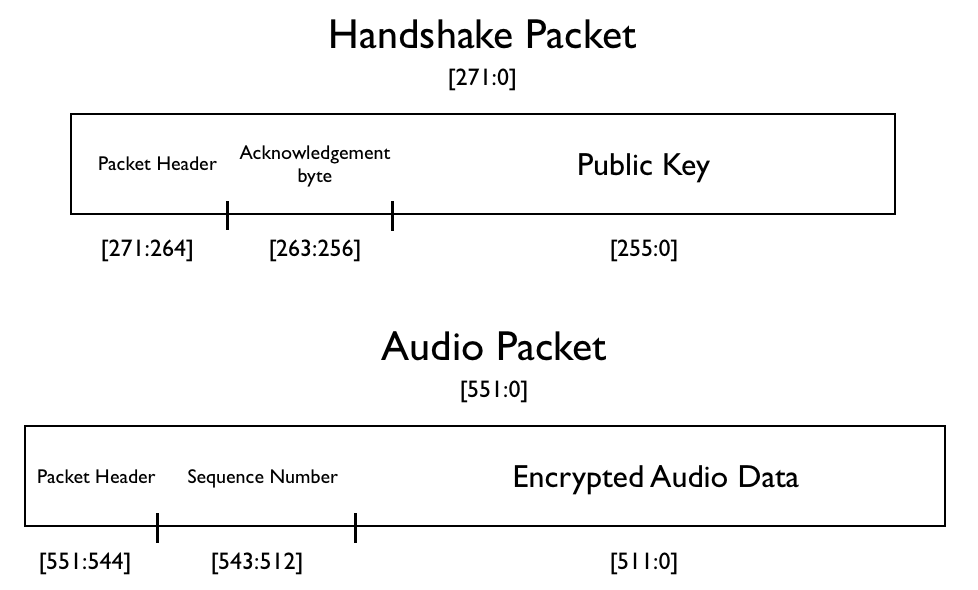
\includegraphics[width=\textwidth]{figs/packets.png}
\centering \caption{The layout of the two types of packets.} 
\end{figure}

Both packets begin with a \emph{packet header}: a string of bits, 10101011, that gets sent over the wire to notify the receiving labkit that transmission of the packet body is about to begin.  \\

The packet body is different for each packet. Handshake packets contain the following components, which make up 272 bits: \\ \\
-An acknowledgement byte (8 bits), depending on whether or not the labkit sending the handshake packet has yet successfully received a handshake packet from its partner. An acknowledgement byte of 01100110 means ``I have not yet received a handshake packet from you'' and an acknowledgement byte of 100110011 means ``I have received a handshake packet from you.''  \\
-The transmitter's unmodified public key (256 bits). Note that because this key is being transmitted over the channel without any modification, an attacker can read the public key; however, due to modern cryptographic hardness conjectures, an attacker with access to both public keys would not be able to find the shared key without running an algorithm that would take years if not millenia to complete (without drastically improving state-of-the-art elliptic-curve-discrete-logarithm algorithms).

Audio packets contain the following components, which make up 552 bits: \\ \\
-A sequence number (32 bits). If this is the $i^{\textrm{th}}$ packet that has been sent over the wire during this phone conversation, then the sequence number would have a value of $i$. Note that because our sequence numbers have a fixed length of 32 bits, no more than $2^{32} \approx $ 4 billion packets can be sent over the wire before the conversation becomes insecure; however, given that we only send 48,000 packets per second over the wire, the phone conversation can last about 100,000 seconds or roughly one day before it is insecure: more than the length of most any phone conversation between two ordinary people. If this design was to be used in a situation where communication was going to last for weeks or months, it would be wise to increase the size of this sequence number to 64 bits. \\
-Encrypted audio data (512 bits). This is the result of a bitwise XOR operation that has been performed between the audio data and the output of the Chacha20 module, which outputs the cryptographic bit-stream. An attacker with access to this audio data and the public keys of both participants in the conversation cannot in a practical way deduce what is being said in the conversation. \\

\section{Buffer Logic}

\emph{Author of section: Adam Yedidia. This module was jointly designed.}

In the code, we did not give this part of the program an actual separate module, but instead put it directly into \verb|labkit.v|. However, both the few lines contained in the execution of the logic and our behavior in how we structured it belie its complexity; this was a very difficult module, both to think about and to execute properly.

The idea of the module is that it must fill buffers with data (be it audio data or handshake data), so that it can be passed, preceded by a packet header, to the serial-port code, which can then send it over the wire. Unfortunately, this is complicated by the fact that if a buffer were to be modified during sending, that could lead to malformed packets being sent: a potential irritant for the user if it happens while audio data is being sent, and potentially catastrophic if it happens during the Diffie-Hellman-Merkle handshake.

To avoid this possibility, the module uses two BRAMs acting as buffers on both the sending and the receiving side, each with 64 slots containing one byte each. While the data from one of the two buffers is being sent over the wire, the other buffer is free to be written into for the next send. Then, when the send on the current buffer finishes, the two buffers switch roles, with the first being ready to be written into and the second relaying its data to the serial port logic to be sent.

\section{Curve25519 Key Exchange}\label{curve25519-key-exchange}

\emph{Author of section: Andres Erbsen}

As classical Diffie-Hellman-Merkle key-exchange requires hundreds of
modular arithmetic operations on multiple-thousand-bit numbers to be
secure, we will be using a modern variation where every modular
multiplication is replaced with the addition of two points on a
carefully chosen elliptic curve{[}@Curve25519{]}. The other relevant
properties of elliptic curve addition are the same as for modular
multiplication, so we will continue to use the classical notation. Even
though one elliptic curve addition uses 10 modular multiplications, the
same level of security can be achieved using numbers that are 10 times
shorter. Numbers that are 10 times shorter are 100 times easier to
multiply, leading to 10 times less chip area and time usage.

The elliptic curve cryptography implementation is the most technically
involved part of this project. {[}@Curve25519{]} gives explicit formulas
for the elliptic curve arithmetic in terms of operations on integers
modulo the prime \(p=2^{255} -19\). Our implementation of the
\texttt{curve25519} module follows the figure presented in the appendix
of that paper and makes use of the properties of our modular arithmetic
modules to provide better performance. The main computation consists of
255 iterations of the elliptic curve Montgomery ladder step operation,
each of which involves 10 modular multiplications and a couple of
additions and subtractions. To allow for a simpler and faster
implementation, the intermediate results are stored as fractions and the
final output fraction is reduced to a scalar at the very end, requiring
modular division. To save area, the circuit has only one copy of the
modular multiplication unit and one add/subtract unit; these are used in
sequence to compute the elliptic curve operation and the division.
Furthermore, as the latency of our modular multiplication unit is twice
as high as the latency of the addition/subtraction unit, but the
throughput is the same, we did our best to keep the multiplication
pipeline active at all times. This results in using 7 255-bit registers
to store the intermediate values, in addition to the internal registers
of the modular arithmetic units. All in all, our implementation requires
less than 70000 cycles to perform an elliptic curve operation (public
key generation or shared key generation). Our implementation is a
trade-off between speed, circuit area, and complexity. We believe that
more careful pipeline management could offer slightly better speeds for
any area, storing the intermediate values of the elliptic curve
operations in block RAM instead of registers would allow for a smaller
area at the expense of speed, and implementing a dedicated modular
division (inversion) unit would allow for significantly better
performance at even larger expense of area.

\subsection{Modular multiplication}\label{modular-multiplication}

We took advantage of the fact that the modulus (\(p=2^{255}-19\)) was
known at the design time, that it is very close to a power of two, and
the availability of 18-by-18-bit multipliers to create implement an
efficient modular multiplication unit. The overall strategy goes as
follows:

\begin{enumerate}
\def\labelenumi{\arabic{enumi}.}
\itemsep1pt\parskip0pt\parsep0pt
\item
  Interpret each 255-bit input as 15 17-bit digits. While it would have
  been possible to use 18-bit digits, choosing 17 greatly simplifies the
  implementation because 255 bits can be evenly divided into 17-bit
  digits but not into 18-bit digits.
\item
  Perform an algorithm similar to schoolbook multiplication, where

  \begin{itemize}
  \itemsep1pt\parskip0pt\parsep0pt
  \item
    During each clock cycle, one row of partial products is computed
  \item
    Each partial product that would eventually overflow the 255-bit
    result because of its position is omitted from the calculation.
  \item
    However, the overflowing partial product is not discarded. As the
    modulus is \emph{not} a power of two, correct for the difference
    between two's complement integer overflow and addition mod \(p\) by
    adding 19 times the number of times the overflow wrapped around to
    the result. Because there must be an empty low order partial product
    slot for each partial product that is statically known to overflow,
    no addition needs to be performed: the just system places 19 times
    the overflowing partial product to the correct slot.
  \end{itemize}
\item
  Cumulatively add up the columns of partial products, but do not handle
  carries between them. The sum of each column has an upper bound of 42
  bits because it is a sum of 17 products of two 17-bit numbers times
  19.
\item
  Handle carries from the two most significant columns, adding the
  number of overflows times 19 to the result as before.
\item
  Handle all remaining carries starting from the least significant
  column and moving towards towards the most significant column. The
  result will be between \(0\) and \(2p\).
\item
  If the result overflows (has a carry of 1), subtract \(p\) from it.
  This is \emph{not} implemented as a separate step. Instead, there are
  two copies of steps 4 and 5, one of which works as described and the
  other subtracts the appropriate digit of \(p\) while handling each
  carry. The correct output is selected amongst the two branches using
  the carry bit.
\end{enumerate}

The breakdown of time usage is roughly as follows: step 2 takes 17
cycles, step 4 takes 1 cycle, and step 5 takes 17 cycles. As the FPGA
provides fast 17-by-17-bit multipliers in dedicated silicon, the main
area usage is due to the the accumulator and operand registers, and the
42-bit adders used for adding up columns and propagating carries.

\subsection{Modular Addition and
Subtraction}\label{modular-addition-and-subtraction}

Addition and subtraction also operate on 15 17-bit digits. While a
larger digit size would have offered superior speed at the submodule
level, we chose to stay consistent with the multiplier implementation
because the addition and subtraction latency is currently not the
bottleneck in the overall system. The general algorithm closely follows
the schoolbook method, and can also be seen as a ripple-carry adder
where a 1-by-1-bit ``full adder'' is replaced with a 17-by-17-bit digit
adder. As in multiplication, we need to ensure that the result of the
operation wraps modulo \(p=2^{255}-19\). Unlike multiplication, the
carry/borrow can only be a single bit, so there is no need for special
handling of carries from higher digits. This allows us to implement a
modular addition (resp. subtraction) of the inputs \(a\) and \(b\) by
first computing both \(a+b\) and \(a+b-p\) (resp. \(a-b\) and \(a-b+p\))
and selecting the one which is in the valid range to output when the
final carry/borrow bit becomes available.

Currently our system has separate circuitry for addition and
subtraction, but only one of them is used at once. We believe that it
would be possible to save some circuit area at negligible speed cost by
having one circuit that allows the operation to be indicated using an
input.

\subsection{Modular Inversion
(Division)}\label{modular-inversion-division}

Our system computes \(\frac{b}{a}\) as \(b\cdot\frac{1}{a}\).
Calculating \(\frac{1}{a}\) is implemented through exponentiation and
multiplication by Fermat's little theorem (\(a^{p-2} = a^{-1}\) mod p),
and exponentiation is done as repeated squaring and multiplication:
\(x^n= x \, ( x^{2})^{\frac{n - 1}{2}} \mbox{ if } n \mbox{ is odd, otherwise } (x^{2})^{\frac{n}{2}}\).
While we are aware of more complicated methods that allow to perform
modular inversion faster, we chose this one because it requires almost
no additional circuit area. Currently, modular inversion accounts for
one fifth of the total modular multiplications and one fourth of the
running time (because the ladder step is pipelined and inversion is
not).

\section{ChaCha20 Stream Cipher}\label{chacha20-stream-cipher}

ChaCha20 is a modern stream cipher. Given a secret key, it provides fast
random access to different positions of \(2^{130}\)-byte keystream which
is XOR-ed with the data to encrypt it. The procedure to compute a
64-byte block of keystream consists of 20 rounds, each of which mutates
a 4-by-4 table of 32-bit words by applying the \emph{quarter round}
function to all columns or all diagonals. A quarter round takes 4 32-bit
inputs and produces 4 32-bit outputs, mixing the bits of the input using
addition, rotation and XOR. Our circuit has four instantiations of the
quarter round module, and one of the twenty rounds is completed each
clock cycle. Finally, the output is computed by adding the initial table
entries to the final table entries (round 21 in our implementation).

This implementation provides good performance (3 bytes/cycle), but the
propagation delay of the circuit is rather large, limiting us to clock
frequencies under 50MHz. In our case it was not an issue (we are using a
27MHz), but a higher frequency implementation would probably need to
pipeline the quarter round function.

\section{Keccak hash function}\label{keccak-hash-function}

We used an open-source Keccak implementation by Homer Hsing, available
at \texttt{opencores.org}. The input is sent to the Keccak module in
chunks of 1 to 4 bytes, the output is a 512-bit high-quality
pseudo-random blob generated as a function of the input. The
implementation we used advertises a speed of 2.4Gbit/s at 100MHz, but we
used it at a much slower rate (less than 1Mbit/s).


\section*{References}\label{references}
\addcontentsline{toc}{section}{References}

1. Diffie, W. and Hellman, M. E. ``\textbf{New Directions in
Cryptography}'' (1976): Available at
\url{http://groups.csail.mit.edu/cis/crypto/classes/6.857/papers/diffie-hellman.pdf}

2. Hellman, M., Diffie, B., and Merkle, R. ``\textbf{Cryptographic
Apparatus and Method}'' (1980): Available at
\url{https://www.google.com/patents/US4200770}

3. Maurer, U. and Wolf, S. ``\textbf{The Diffie--Hellman Protocol}''
\emph{Designs, Codes and Cryptography} 19, no. 2-3 (2000): 147--171.
doi:\href{http://dx.doi.org/10.1023/A:1008302122286}{10.1023/A:1008302122286},
Available at \url{http://dx.doi.org/10.1023/A\%3A1008302122286}

4. Bernstein, D. J. ``\textbf{ChaCha, a Variant of Salsa20}'' (2008):
Available at \url{http://cr.yp.to/chacha/chacha-20080128.pdf}

5. Bernstein, D. J. ``\textbf{Attacks Against ChaCha20}'' (2008):
Available at \url{http://cr.yp.to/streamciphers/attacks.html\#chacha6}

6. NIST. ``\textbf{SHA-3 Submission Requirements}'' (2007): Available at
\url{http://csrc.nist.gov/groups/ST/hash/sha-3/Submission_Reqs/algo_specs.html}

7. ``\textbf{BLAKE Cryptanalysis}'' Available at
\url{https://131002.net/blake/\#cr}

8. Bernstein, D. J. ``\textbf{Curve25519: New Diffie-Hellman Speed
Records}'' \emph{Public key cryptography - pKC 2006, 9th international
conference on theory and practice of public-key cryptography} 3958,
(2006): 207--228.
doi:\href{http://dx.doi.org/10.1007/11745853_14}{10.1007/11745853\_14},
Available at
\url{http://www.iacr.org/cryptodb/archive/2006/PKC/3351/3351.pdf} 


\end{document}
